\documentclass[11pt]{amsart}
\usepackage{geometry}                % See geometry.pdf to learn the layout options. There are lots.
\geometry{letterpaper}                   % ... or a4paper or a5paper or ...
%\geometry{landscape}                % Activate for for rotated page geometry
%\usepackage[parfill]{parskip}    % Activate to begin paragraphs with an empty line rather than an indent
\usepackage{booktabs}
\usepackage{graphicx}
\usepackage{amssymb}
\usepackage{epstopdf}
\usepackage{caption}
\usepackage{subcaption}
\usepackage{commath}
\DeclareGraphicsRule{.tif}{png}{.png}{`convert #1 `dirname #1`/`basename #1 .tif`.png}

\usepackage{verbatim}

% Declare commands
\newcommand{\mat}[1]{\mathbf{#1}}
\DeclareMathOperator*{\argmax}{arg\,max}

\title{CS 181 -- Final Project}
\author{Casey Grun, Sam Kim, Rhed Shi (\textrm{SrcTeam})}
%\date{}                                           % Activate to display a given date or no date

\begin{document}
\maketitle

% =============================================================================
\section{Overview}

In this project, our challenge was to develop an agent to play a variant of Pac-man, where several aspects of the game's behavior were uncertain. We were tasked with developing an agent that would accumulate as many points as possible by eating ``good'' ghosts, or by eating the ``bad'' ghost after a non-placebo capsule. However, our agent would not know \emph{a priori} which ghosts were good and which was bad, nor would it know which capsules would allow the bad ghost to be eaten (and which were placebos). Finally, Pac-man would lose half a point every turn due to hunger, and would lose a large number of points if caught by the bad ghost without having eaten a capsule.

We therefore had four challenges for this assignment:
\begin{description}
	\item[Capsule clustering] --- Because the capsule data were not labelled nor the distributions of capsule feature vectors known, we used unsupervised clustering techniques to group cluters tegoether such that we can identify placebo versus non-placebo capsules.
	\item[Ghost classification] --- We used various supervised learning techniques and chose the best one for classifying the latent class of the ghosts. We additionally modified the data to also classify ghosts as either bad or good.
	\item[Score Regression] --- Based on the latent class of the ghost, we used linear regression to predict the juiciness of the ghost. Each ghosts class has its own different model governing its juiciness level and so it would be more accurate to apply linear regression on ghosts with the same class. 
	\item[Agent development] --- We used reinforcement learning to attempt to train an optimal agent strategy, incorporating information from the ghost and capsule classification data. We also built several agents using hand-coded strategies that incorporated the capsule and ghost classification 
\end{description}

% =============================================================================
\section{Capsule classification}

The features vectors of the capsules have only 3 features, so the first step we took was plotting the feature vectors in 3 dimensions to visualize the data and hopefully gain an intuitive understanding of the data.

\begin{figure}[h]
	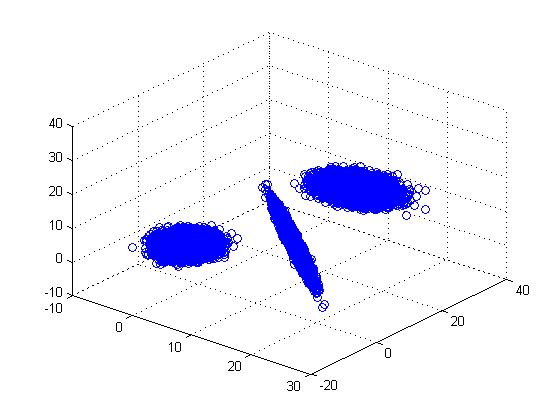
\includegraphics[width=10cm]{capsuleCluster.png}
	\caption{Plot of the capsule feature vectors.}
	\label{fig:capsules}
\end{figure}

As we can see from Figure ~\ref{fig:capsules}, the capsules seem to be split into 3 clusters, each of which resemble a Gaussian distribution. Additionally, plotting the labeled capsules using the \texttt{getGoodCapsuleExamples()} function shows that all the examples for a particular random seed come from a single cluster, confirming our intuition. We test both K-Means++ and Gaussian Mixture Models to cluster the data.

\begin{figure}
	\begin{subfigure}{\textwidth}
		\centering		
		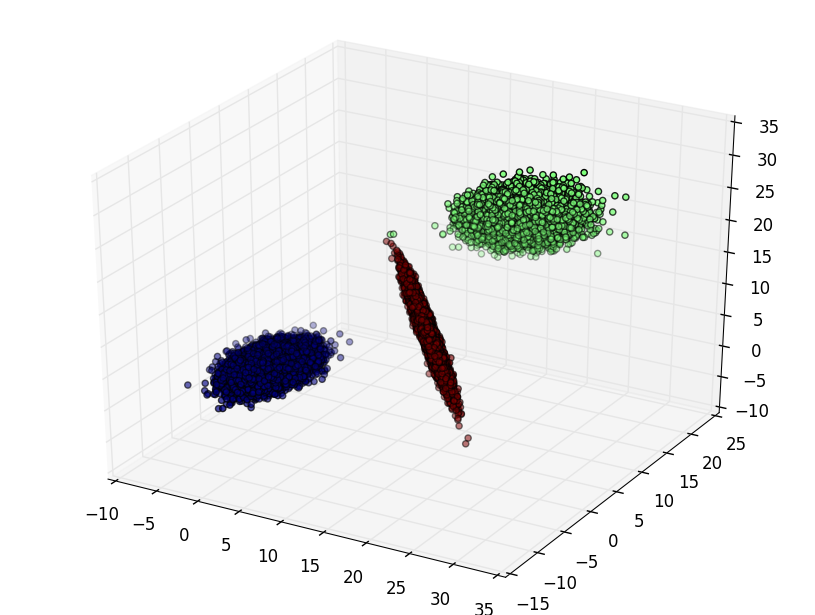
\includegraphics[width=0.8\textwidth]{capsule_k_means_plot.png}
		\caption{K-Means++.}
	\end{subfigure}
	\begin{subfigure}{\textwidth}
		\centering
		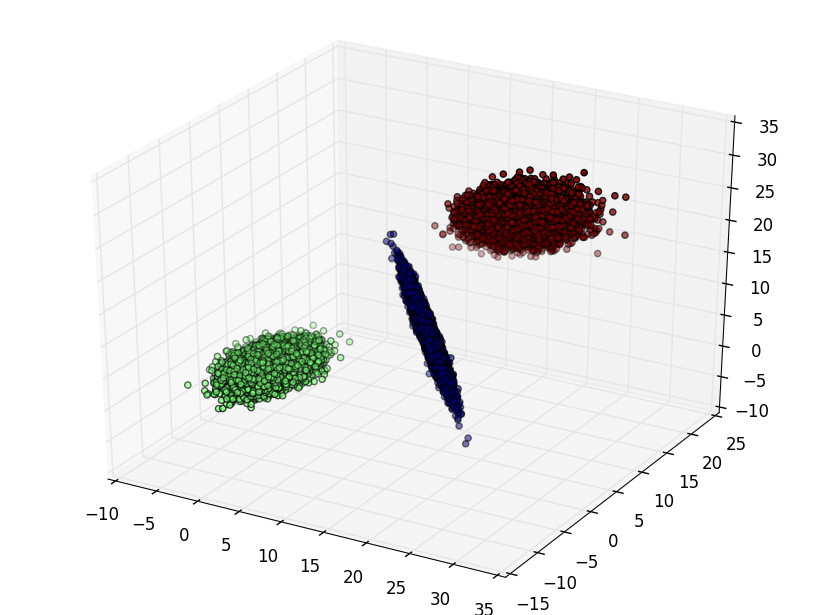
\includegraphics[width=0.8\textwidth]{capsule_gauss_plot.png}
		\caption{Gaussian Mixture Models}
	\end{subfigure}
	\caption{Clustering of capsule data with 3 clusters. Colors correspond to labels, which are ordered arbitrarily.}
	\label{fig:clustering}
\end{figure}

Figure ~\ref{fig:clustering} shows the results of clustering using both K-Means++ and Gaussian Mixture Models. 
The K-Means++ algorithm runs multiple times with random initializations, choosing the configuration that has the lowest error as the final answer. For the K-Means++, most of the points seem to be in their respective clusters, but we see several points in the center cluster that are colored as green, although visually they seem like they should be colored red. This is because the K-Means error function only considers distance to a cluster mean, rather than distance to other cluster points. 
Gaussian Mixture Models are able to use non-diagonal covariance matrices, which allow more flexibility in the distribution of points within each cluster. Thus, from the figure, it appears that all the points have been clustered correctly.

To decide if a given capsule is a placebo or not, we test if it is in the same cluster as the majority of the example good capsules given by the \texttt{getGoodCapsuleExamples()} function.

\pagebreak

% =============================================================================
\section{Ghost classification}

The feature vectors for the ghosts are 13-dimensional. The data sets generated gave feature vectors paired with the ghost latent class, the score, and the quadrant. First, we tried to determine the latent class of the ghosts based on their feature vectors (multi-classification). Next we tried separately to simply classify the ghosts into good or bad (binary classification). By definition, having a latent class of 5 meant the ghost was bad and having a latent class of 0, 1, 2, or 3 meant the ghost was good. However, we hypothesized that the binary classification would be (computationally) easier, and may be the only necessary information for some agent strategies.

We used three major approaches to classify the ghosts and compared them to each other: one vs. rest, one vs. one, and logistic regression. These were taken from the scikit-learn \texttt{multiclass} and \texttt{linear\_model} packages.

To test our approach, we used 10-fold cross validation on a data set with around 4000 data points. For our cross validation, we randomly split the data set each time into 10 equally sized sets and trained on 9 out of 10 data sets and tested on 1 out of 10 data set. 


\begin{figure}
	\centering
	\begin{subfigure}{0.49\textwidth}
		\centering		
		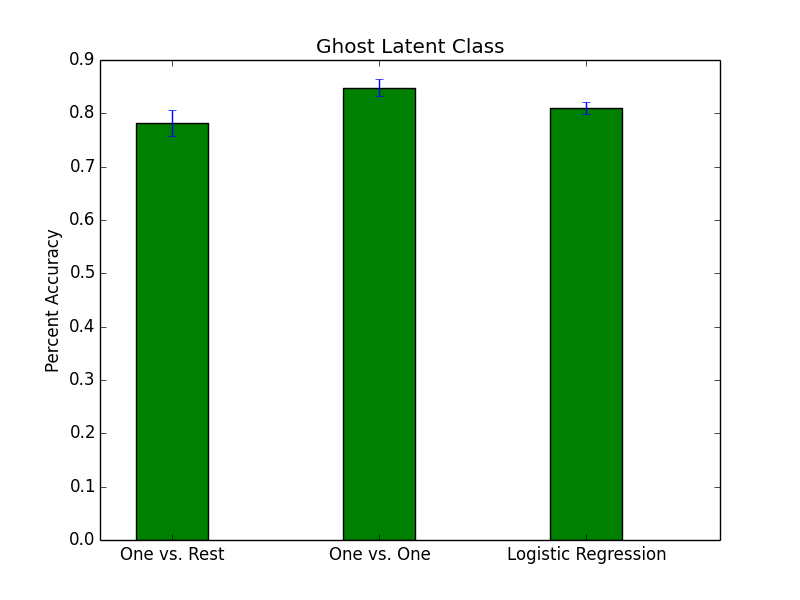
\includegraphics[width=\textwidth]{ghost_latent_class.png}
		\caption{Latent class classification.}
		\label{fig:latent_class}
	\end{subfigure} %
	\begin{subfigure}{0.49\textwidth}
		\centering
		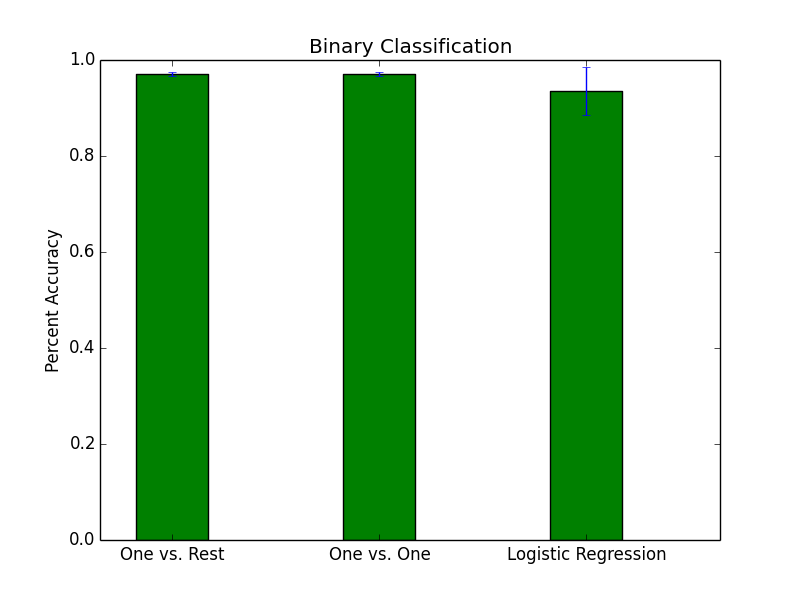
\includegraphics[width=\textwidth]{binary_classification.png}
		\caption{Binary classification for good and bad ghosts.}
		\label{fig:binary}
	\end{subfigure}
	\caption{Ghost classification using three methods: one vs. rest, one vs. one, and logistic regression.}
	\label{fig:classification}
\end{figure}

\begin{comment}
\begin{table}[b]
\caption{10-fold cross validation for classification of latent class of the ghosts on data set using one vs. rest classifier, one vs. one classifier, and logistic regression.}
\centering
\begin{tabular}{c  c  c  c}
\hline \hline \\ 
$k$-fold & One vs. Rest & One vs. One & Logistic Regression \\ [0.5ex]
\hline \\ 
1 & 0.796663 & 0.862176 & 0.817058 \\
2 & 0.785538 & 0.831891 & 0.809023 \\
3 & 0.78801 & 0.86403 & 0.825093 \\
4 & 0.721261 & 0.818294 & 0.789246 \\
5 & 0.800989 & 0.854141 & 0.805933 \\
6 & 0.812114 & 0.843016 & 0.814586 \\
7 & 0.755102 & 0.831169 & 0.792208 \\
8 & 0.774273 & 0.858998 & 0.8188 \\
9 & 0.785405 & 0.845393 & 0.808287 \\
10 & 0.796537 & 0.87384 & 0.823129 \\
\hline \\
Avg. & 0.781589 & 0.848295 & 0.810336 \\
Std. & 0.024949 & 0.016554 & 0.011468 \\
\hline
\end{tabular}
\label{table:latent_class}
\end{table}
\end{comment}

\subsection{Latent Class}

For our latent class ghost classification, we used one vs. rest, one vs. one, and logistic regression strategies. In one vs. rest we come up with a classifier for each latent class compared to the rest of the data. In one vs. one we come up with a classifier for each pair of latent classes to differentiate them. For both of these classification strategies, we used a linear SVC (support vector classification) from the scikit-learn \texttt{svm} package, as well as logistic regression from the \texttt{linear\_model} package. As shown in Figure~\ref{fig:latent_class}, the one vs. one classifier using linear SVC performed the best on our cross validation platform, followed by logistic regression. The one vs. one classifier with linear SVC had an average of 85\% accuracy.

\subsection{Binary Classification}

For our binary classification of good ghosts and bad ghosts, we simply modified our data set such that all ghosts with latent class 5 were relabeled as 1, and all ghosts with latent classes 0, 1, 2, or 3 were relabeled as 0. Then we applied one vs. one, one vs. rest, and logistic regression. However, this time instead of using linear SVC as the classification boundary, we used the regular SVC with a radial basis function kernel:
$$ K(x,x') = \text{exp}\left(-\frac{|| x - x' ||_2^2}{2\sigma^2}\right).$$

\begin{comment}
\begin{table}[b]
\caption{10-fold cross validation for binary classification of good ghosts and bad ghosts on data set using one vs. rest classifier, one vs. one classifier, and logistic regression.}
\centering
\begin{tabular}{c  c  c  c}
\hline \hline [0.5ex]
$k$-fold & One vs. Rest & One vs. One & Logistic Regression \\ [0.5ex]
\hline
1 & 0.967244 & 0.967244 & 0.870828 \\
2 & 0.969098 & 0.969098 & 0.851669 \\
3 & 0.966007 & 0.966007 & 0.854759 \\
4 & 0.972188 & 0.972188 & 0.86403 \\
5 & 0.972806 & 0.972806 & 0.872064 \\
6 & 0.966625 & 0.966625 & 0.858467 \\
7 & 0.971552 & 0.971552 & 0.87384 \\
8 & 0.975881 & 0.975881 & 0.866419 \\
9 & 0.975263 & 0.975263 & 0.888064 \\
10 & 0.970934 & 0.970934 & 0.84663 \\
\hline
Avg. & 0.97076 & 0.97076 & 0.935399 \\
Std. & 0.003289 & 0.003289 & 0.05053 \\
\hline
\end{tabular}
\label{table:binary}
\end{table}
\end{comment}

As shown in Figure~\ref{fig:binary}, this dramatically improved the performance of both one vs. one and one vs. rest classification. Logistic regression on this binary classification problem also improved from before. The best classification method was a tie between the one vs. one and one vs. rest method with about 97\% accuracy.

% =============================================================================
\section{Score Regression}

Given that we were able to classify ghosts into their latent class, we decided to perform linear regression on the scores conditioned on the latent class of the ghost. Thus, we split the data set into each of the latent classes for good ghosts (the score for the bad ghost with latent class 5 is already determined as +1200 or -1000 by the rules of the game). 

As we can see from Figure~\ref{fig:score}, the results are mixed with the most accurate predictions for Latent Class 2 and the least accurate predictions for Latent Class 0. The coefficients of determination ($R^2$) shown in the figure are given by:

$$ 1 - \frac{\text{residual sum of squares}}{\text{total sum of squares}} = 1 - \frac{\sum_i (y_i - x_i w)^2}{\sum_i (y_i - \bar{y}_i)^2}$$ 

where $x_i w_i$ represents a predicted value for some $y_i$, based on a feature vector $x_i$ and a weight vector $w$.

\begin{figure}[b]
	\centering
	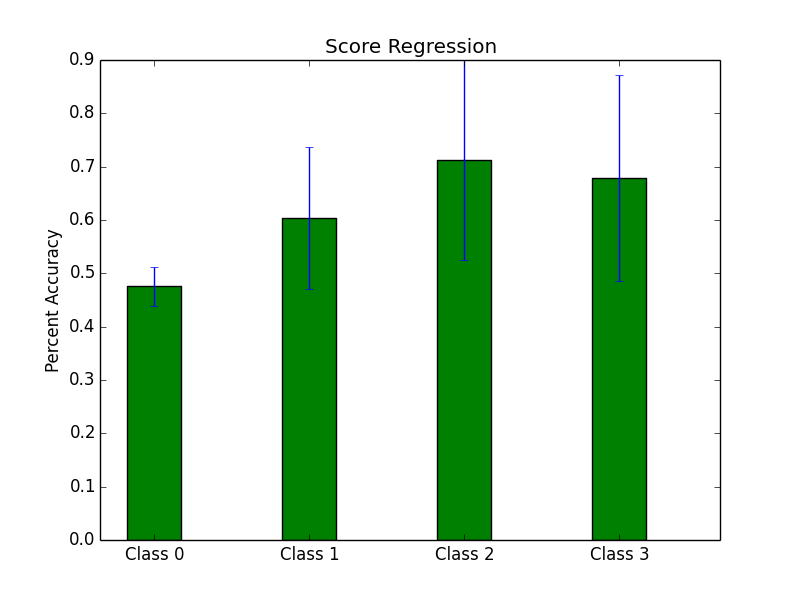
\includegraphics[width=0.7\textwidth]{score_regression.png}
	\caption{Latent class conditional score regression using Bayesian ridge regression.}
	\label{fig:score}
\end{figure}

\begin{comment}
\begin{table}[t]
\caption{10-fold cross validation latent class conditional score regression on ghosts.}
\centering
\begin{tabular}{c  c  c  c  c}
\hline \hline
$k$-fold & Latent Class 0 & Latent Class 1 & Latent Class 2 & Latent Class 3 \\ [0.5ex]
\hline
1 & 0.451262 & 0.73688 & 0.922407 & 0.615995 \\
2 & 0.445523 & 0.787039 & 0.939079 & 0.722243 \\
3 & 0.497986 & 0.767327 & 0.920362 & 0.660554 \\
4 & 0.551044 & 0.689065 & 0.942813 & 0.329324 \\
5 & 0.495902 & 0.699544 & 0.942473 & 0.67256 \\
6 & 0.418256 & 0.701683 & 0.936595 & 0.161031 \\
7 & 0.500379 & 0.728969 & 0.918327 & 0.645223 \\
8 & 0.476065 & 0.721426 & 0.935348 & 0.701346 \\
9 & 0.433965 & 0.714542 & 0.916941 & 0.604004 \\
10 & 0.483605 & 0.783922 & 0.895121 & 0.71846 \\
\hline
Avg. & 0.475399 & 0.604219 & 0.711795 & 0.679615 \\
Std. & 0.037151 & 0.13359 & 0.187379 & 0.19308 \\
\hline
\end{tabular}
\label{table:score}
\end{table}
\end{comment}

\subsection{Bayesian Ridge Regression}

We used Bayesian ridge regression to estimate the juiciness score of the ghosts. Bayesian ridge regression is a probabilistic model on ridge regression which minimizes the penalized residual sum of squares:
$$ \min_w ||Xw - y||_2^2 + \alpha||w||_2^2,$$
where $\alpha$ is the complexity parameter or regularization parameter. The probabilistic model for the Bayesian ridge regression assumes that $y$ is a Gaussian distributed around a mean $Xw$:
$$ p(y | X, w, \alpha) = \mathcal{N}(y  | Xw, \alpha) $$ 
with the prior for the $w$ is given by
$$ p(w | \lambda) = \mathcal{N}(w | 0, \lambda^{-1}\mathbb{I_p}) $$
and the prior distribution for $\alpha$ and $\lambda$ given by gamma distributions. We used default values for $\alpha_1 = \alpha_2 = \lambda_1 = \lambda_2 = 1 \times 10^{-6}$.

% =============================================================================
\section{Agents}

We implemented several agents---some took advantage of reinforcement learning, while some employed hand-coded strategies. We did not have time to incorporate the ghost ``juiciness'' regression results into any of these strategies, but the agents all drew upon the capsule clustering and ghost classification results described above.

% -----------------------------------------------------------------------------
\subsection{Reinforcement Learning Agents}

In order to explore whether reinforcement learning could be used to train an optimal strategy, we implemented a series of agents that performed reinforcement learning using Q-learning.

Briefly, our agent begins with an estimate of $Q(s,a)$. Upon taking an action $a$ (during epoch $t$), recieving a reward $r$, and observing a transition from $s$
to $s'$, the agent updates our running estimate of $Q(s,a)$ as follows:
$$Q(s,a) \gets Q(s,a) + \alpha_k(s,a) \left[ (r + \gamma \max_{a' \in \mathcal{A}} Q(s', a')) - Q(s,a) \right].$$

We obtained best results when the learning rate $\alpha$ was set to 0.01 for the first 1000 epochs, after which it was set to 0.001. The optimal value for the discount factor $\gamma$ was about 0.4; these were determined by coordinate descent. 

A key challenge was determining how the many-dimensional, partially-observable game state could be discretized into a single, discrete state representation $s$. We therefore experimented with several ``basis functions'' for representing the state space. We built three different agents that utilized different basis function representations:

\begin{description}
	\item[GhostPositionAgent] --- $s = ((p_x, p_y), (g_x, g_y), (b_x, b_y), (c_x, c_y), h)$ where $(p_x, p_y)$ is the position of Pac-man, $(g_x, g_y)$ is the position of the closest good ghost $(b_x, b_y)$ is the position of the bad ghost, $(c_x, c_y)$, is the position of the nearest non-placebo capsule, and $h$ is 1 if Pac-man has eaten a capsule (e.g. the bad ghost is currently scared). The positions $(p_x, p_y), (g_x, g_y), (b_x, b_y), (c_x, c_y)$ were each binned into $n$ bins, such that there were $n^{2 * 4} * 2$ possible states. This agent attempts to learn a direction to move for each configuration.
	\item[LocalNeighborhoodAgent] --- $s = ((g_x, g_y), (b_x, b_y), (c_x, c_y), h)$. Similar to GhostPositionAgent; however, positions are stored relative to Pac-man himself. Each dimension is binned into one of $n$ values; if one of the objects is a distance of more than $r$ away from Pac-man in one dimension, it is classified in the most distant bin in that dimension. This agent attempts to reduce the effective dimensionality of the GhostPositionAgent, but maintains the directional information lost by the GoodBadCapsuleDistanceAgent. This agent attempts to learn a direction to move for each configuration.
	\item[GoodBadCapsuleDistanceAgent] --- $s = (g, b, c, h)$ where $g$ is the distance to the nearest good ghost, $b$ is the distance to the bad ghost, $c$ is the distance to the nearest non-placebo capsule, and $h$ is 1 if Pac-man has eaten a capsule (e.g. the bad ghost is currently scared). Each of the distances $g$, $b$, and $c$ were sorted into one of $n$ bins, where $n = 5$, such that the size of the state space was $n^3 * 2$. Unlike the other two agents, this agent attempts to learn \emph{which object to pursue} (the good ghost, the bad ghost, or the capsule). Once the learner has selected the object to pursue, the agent will move in whichever legal direction minimizes the distance to the target.  
\end{description}

In an attempt to improve the rate of convergence, recognizing in particular that Q-learning is much slower to propagate negative rewards than positive rewards, we implemented two learners that were ``seeded'' with initial values, based on our knowledge about expected rewards for various actions (according to the game rules):

\begin{description}
	\item[SeededGoodBadCapsuleDistanceAgent] --- Same as GoodBadCapsuleDistanceAgent; however, chasing the bad ghost without the capsule was assigned $Q = -1200$, regardless of the distance.
	\item[SeededLocalNeighborhoodAgent] --- Same as LocalNeighborhoodAgent; however, any action which moved towards the bad ghost without the capsule was assigned $Q = -1200$ if the bad ghost was within the radius $r$ of Pac-man.
\end{description}

% -----------------------------------------------------------------------------
\subsection{Hand-coded Agents}

We implemented 3 different hard-coded strategies that relied on capsule clustering and ghost classification algorithms, and did not rely on training the behavior.
\begin{description}
	\item[SafeAgent] If there are no scared ghosts, then chases the closest non-placebo capsule, actively avoiding all ghosts along the way. If the ghost is scared, then the agent goes after any nearby ghost regardless of its classification, eating capsules along the way. 
	\item[AnyGhostAgent] If there are no scared ghosts, then chases the closest non-placebo capsule, eating good ghosts along the way if it does not have to stray far from its path. If the ghost is scared, then the agent goes after any nearby ghost regardless of its classification, eating capsules along the way. 
	\item[BadGhostAgent] If there are no scared ghosts, then chases the closest non-placebo capsule, actively avoiding all ghosts along the way. If the ghost is scared, then it chases the scared ghost, eating capsules and good ghosts along the way if it does not have to stray far from its path.
\end{description}

% -----------------------------------------------------------------------------
\subsection{Agent comparison}

Figs. \ref{fig:agents-finals} and \ref{fig:agents-trajectories} compare the performance of the various agents that we implemented, as well as two test agents that serve as controls:
\begin{description}
	\item[CapsuleAgent] Always pursues the nearest capsule.
	\item[GhostAgent] Always pursues the bad ghost (regardless of capsule status).
\end{description} 

\begin{figure}
	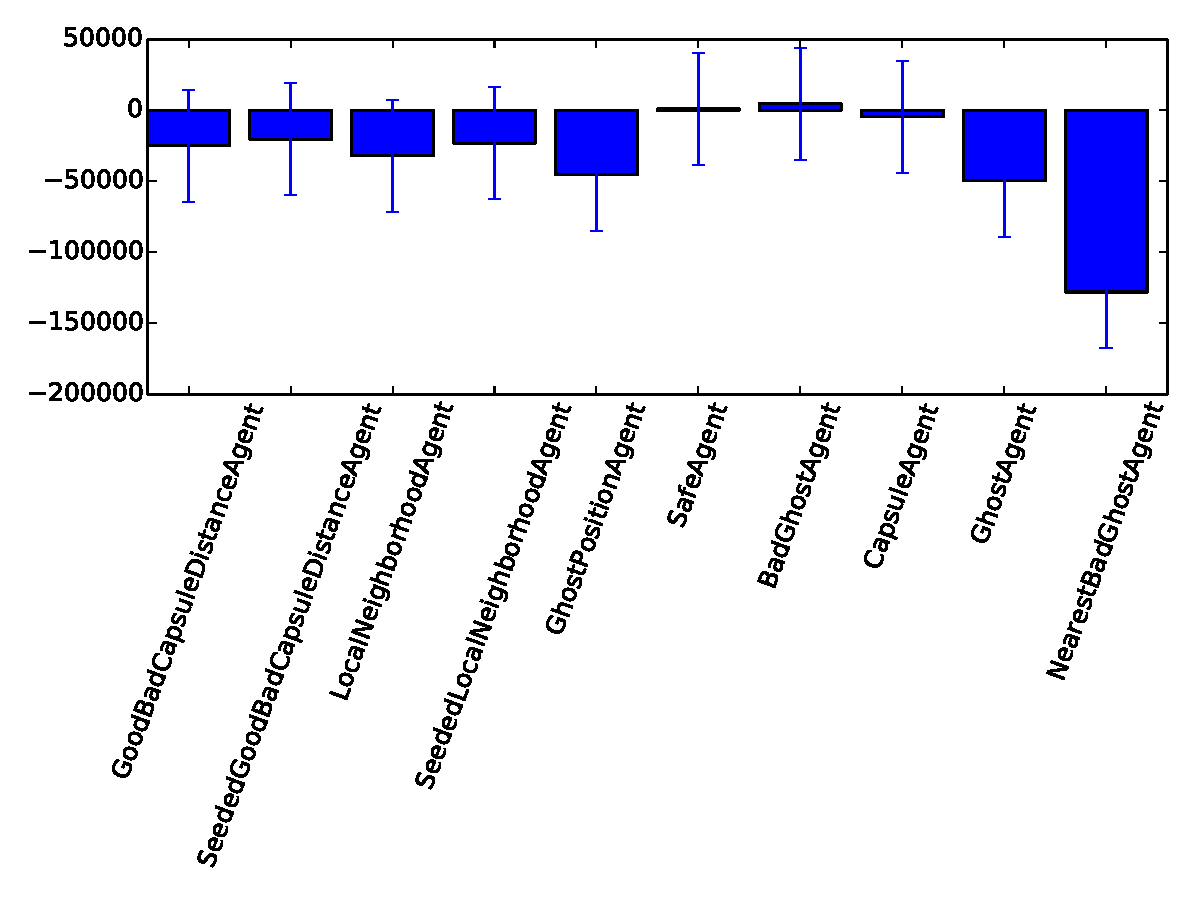
\includegraphics[width=\textwidth]{agents-finals.pdf}
	\caption{Final scores (after 1000 game steps) for each agent (mean $\pm$ std. dev., $n = 10$ games for each agent)}
	\label{fig:agents-finals}
\end{figure}

As can be seen from Fig. \ref{fig:agents-finals}, the three hand-coded agents performed much better than the reinforcement-learning agents (although the seeded agents did better than the non-seeded reinforcement learning agents). We suspect that further tuning of the learning rate may have helped the reinforcement learning agents converge to an optimal strategy. Another problem was that our ghost-classification performance improved significantly very close to the deadline---before we were able to re-train our reinforcement agents. Therefore the reinforcement agents may have evolved strategies that were overly conservative due to spurious punishments when pursuing the bad ghost (that had been mis-classified as the good ghost).

Examining Fig. \ref{fig:agents-trajectories} provides some insights into the failure modes of the poorly-performing agents. It can be seen that poorly-perfoming agents do not simply die of attrition, but repeatedly experience 1000-point losses (presumably due to bad ghost encounters). This seems to suggest that either: the bad ghost is being repeatedly mis-classified, the agents are pursuing the bad ghost (despite not having a capsule---presumably due to a failure to propagate negative reward), or the agent, in pursuit of another ghost or capsule, accidentally runs into the bad ghost.

Most of the failure modes of the hard-coded strategy ghosts had to do with poor path-finding, as we had only implemented a simple behavior to move towards the target when legal and make a random move otherwise, rather than actively routing around obstacles and bad ghosts. This was especially detrimental in ``local minima'' when the bad ghost would hover near the good capsule.

\begin{figure}
	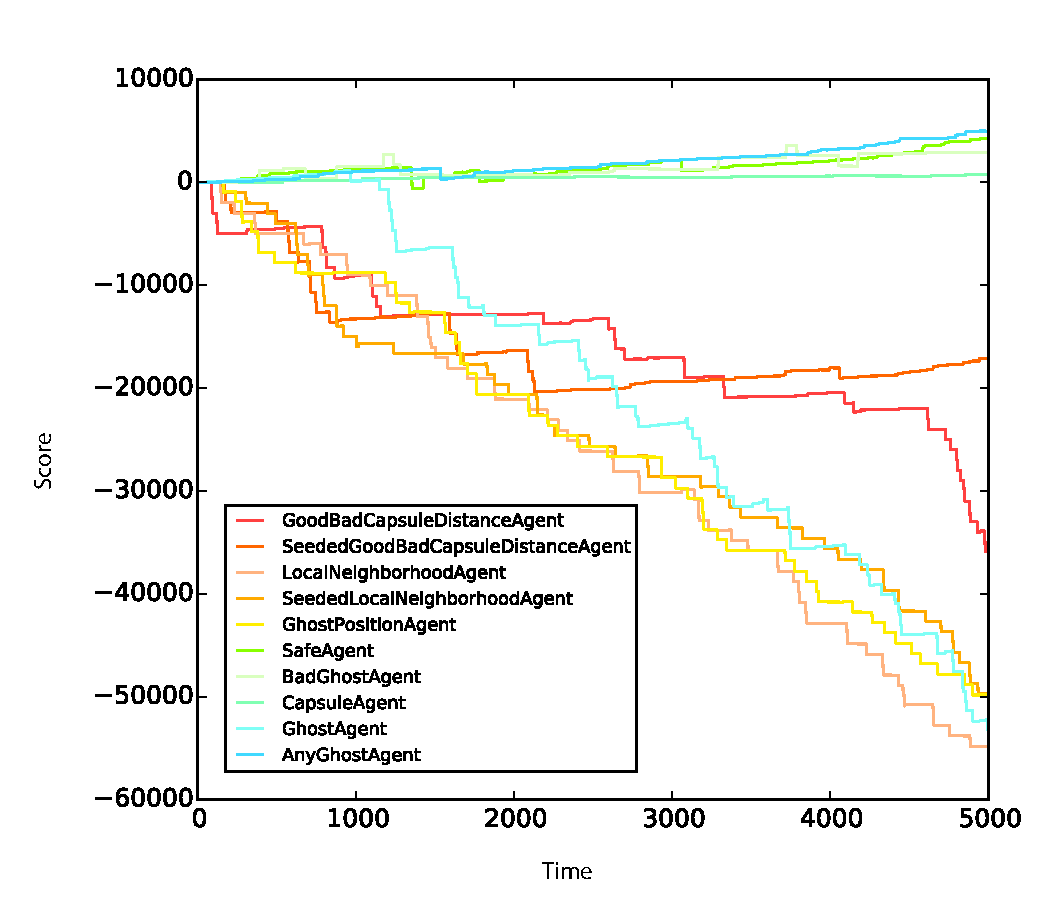
\includegraphics[width=\textwidth]{agents-trajectories.pdf}
	\caption{Representative trajectories of each agents: game step vs. score.}
	\label{fig:agents-trajectories}
\end{figure}


% =============================================================================
\section{Conclusion}

Ultimately, our most successful approaches were the hand-coded strategies. This is somewhat unsurprisingly, as those strategies were able to incorporate the information gleaned by the offline learning techniques, but pursued a nearly-optimal strategy based on knowledge of the game mechanics (something from which the reinforcement learning agents did not benefit). Improvements in the reinforcement learning agents' performance may have been achieved by tweaking the learning rate and the discretization parameters. Further improvements in the hand-coded strategies could be obtained by performing class-conditional regression on the ghosts' feature vectors in order to predict the ``juiciness'' of each ghost (and therefore make more considered and less-opportunistic decisions about which ghost/capsule to pursue). Similarly, probabilistic classification of the capsules could have been incorporated into decision-making (for instance, the confidence in a classification or juiciness prediction could determine which of several options was pursued). This type of decision-making may be better-suited to continuous formulations of reinforcement learning. These would be appropriate avenues for future study.
\end{document}